\documentclass[12pt,a4paper]{article}

% ─── Page Layout ───────────────────────────────────────────────────────────────
\usepackage[a4paper, margin=0.8in, headheight=14pt]{geometry}

% ─── Fonts (XeLaTeX) ───────────────────────────────────────────────────────────
\usepackage{fontspec}
\usepackage{unicode-math}
\setmainfont{TeX Gyre Pagella}
\setmonofont[Scale=0.88]{TeX Gyre Cursor}
\setmathfont{Latin Modern Math}

% ─── Packages ──────────────────────────────────────────────────────────────────
\usepackage{xcolor}
\usepackage{colortbl}
\usepackage{titlesec}
\usepackage{enumitem}
\usepackage{tabularx}
\usepackage{booktabs}
\usepackage{array}
\usepackage{amsmath}
\usepackage{tikz}
\usetikzlibrary{shapes.geometric, arrows.meta, positioning, calc, fit, decorations.pathreplacing}
\usepackage{tcolorbox}
\tcbuselibrary{skins, breakable}
\usepackage{hyperref}
\usepackage{fancyhdr}
\usepackage{graphicx}
\usepackage{microtype}
\hyphenpenalty=10000
\exhyphenpenalty=10000
\sloppy
\usepackage{caption}
\usepackage{setspace}
\usepackage{multirow}
\usepackage{tocloft}

% ─── Q&A helper ────────────────────────────────────────────────────────────────
\newcommand{\Q}[1]{\textbf{#1}\par\noindent\ignorespaces}

% ─── Colour Palette ────────────────────────────────────────────────────────────
\definecolor{myred}{RGB}{196,30,58}
\definecolor{mydark}{RGB}{30,30,50}
\definecolor{mygreen}{RGB}{14,120,80}
\definecolor{myteal}{RGB}{0,130,140}
\definecolor{myamber}{RGB}{180,100,0}
\definecolor{mypurple}{RGB}{100,30,160}
\definecolor{mygray}{RGB}{246,247,249}
\definecolor{mgframe}{RGB}{180,185,200}
\definecolor{watermark}{RGB}{145,150,170}
\definecolor{hdrred}{RGB}{250,232,235}
\definecolor{hdrgreen}{RGB}{220,244,233}
\definecolor{hdrteal}{RGB}{220,242,244}
\definecolor{hdramber}{RGB}{253,242,215}
\definecolor{hdrpurple}{RGB}{238,228,255}
\definecolor{hdrgray}{RGB}{238,240,245}
\definecolor{rowalt}{RGB}{250,251,253}

% ─── Section Formatting ────────────────────────────────────────────────────────
\titleformat{\section}
  {\large\bfseries\color{myred}}{\thesection.}{0.5em}{}
  [\vspace{1pt}{\color{myred}\rule{\linewidth}{0.8pt}}]
\titleformat{\subsection}
  {\normalsize\bfseries\color{myteal}}{\thesubsection}{0.5em}{}
\titlespacing*{\section}{0pt}{18pt}{7pt}
\titlespacing*{\subsection}{0pt}{11pt}{4pt}

% ─── Paragraph ─────────────────────────────────────────────────────────────────
\setlength{\parindent}{0pt}
\setlength{\parskip}{4pt}

% ─── TOC Styling ───────────────────────────────────────────────────────────────
\renewcommand{\cfttoctitlefont}{\large\bfseries\color{myred}}
\renewcommand{\cftaftertoctitle}{\par\noindent{\color{myred}\rule{\linewidth}{0.8pt}}}
\setlength{\cftbeforetoctitleskip}{0pt}
\setlength{\cftaftertoctitleskip}{6pt}
\renewcommand{\cftsecfont}{\normalsize\bfseries\color{mydark}}
\renewcommand{\cftsecpagefont}{\normalsize\bfseries\color{mydark}}
\renewcommand{\cftsecleader}{\cftdotfill{\cftdotsep}}
\setlength{\cftbeforesecskip}{7pt}
\renewcommand{\cftsubsecfont}{\small\color{mydark}}
\renewcommand{\cftsubsecpagefont}{\small\color{mydark}}
\setlength{\cftbeforesubsecskip}{3pt}
\setlength{\cftsubsecindent}{1.4em}

% ─── Table helpers ─────────────────────────────────────────────────────────────
\renewcommand{\arraystretch}{1.45}
\setlength{\tabcolsep}{6pt}
\arrayrulecolor{mydark}
\newcolumntype{B}[1]{>{\small\bfseries\raggedright\arraybackslash}m{#1}}
\newcolumntype{Y}{>{\small\raggedright\arraybackslash}X}
\renewcommand{\tabularxcolumn}[1]{m{#1}}

% ─── Header / Footer ───────────────────────────────────────────────────────────
\pagestyle{fancy}
\fancyhf{}
\fancyhead[L]{\small\color{myred}\textbf{PE-EC603A}\;\color{mydark}--- Introduction to MEMS}
\fancyhead[R]{\small\color{myteal}\textbf{Module 2 Notes}}
\fancyfoot[C]{\small\color{mydark}\thepage}
\fancyfoot[R]{\small\color{watermark}\textit{\copyright\ Biraj}}
\renewcommand{\headrulewidth}{0.5pt}
\renewcommand{\footrulewidth}{0.3pt}

% ─── Hyperref ──────────────────────────────────────────────────────────────────
\hypersetup{
  colorlinks=true, linkcolor=myteal, urlcolor=myteal,
  pdfauthor={Biraj Sarkar},
  pdftitle={PE-EC603A --- Module 2 Notes}
}

% ─── tcolorbox styles ──────────────────────────────────────────────────────────
\tcbset{
  tikzbox/.style={
    colback=mygray, colframe=mgframe, boxrule=0.6pt, arc=4pt,
    left=8pt, right=8pt, top=6pt, bottom=6pt,
    colbacktitle=mgframe, coltitle=mydark,
    fonttitle=\small\bfseries
  },
  defbox/.style={
    colback=hdrgreen, colframe=mygreen, boxrule=0.8pt, arc=4pt,
    left=9pt, right=9pt, top=6pt, bottom=6pt,
    colbacktitle=mygreen, coltitle=white,
    fonttitle=\small\bfseries
  },
  formulabox/.style={
    colback=hdrteal, colframe=myteal, boxrule=0.8pt, arc=4pt,
    left=9pt, right=9pt, top=7pt, bottom=7pt,
    colbacktitle=myteal, coltitle=white,
    fonttitle=\small\bfseries
  },
  examplebox/.style={
    colback=hdramber, colframe=myamber, boxrule=0.8pt, arc=4pt,
    left=9pt, right=9pt, top=6pt, bottom=6pt,
    colbacktitle=myamber, coltitle=white,
    fonttitle=\small\bfseries
  },
  masonbox/.style={
    colback=hdrpurple, colframe=mypurple, boxrule=0.8pt, arc=4pt,
    left=9pt, right=9pt, top=6pt, bottom=6pt,
    colbacktitle=mypurple, coltitle=white,
    fonttitle=\small\bfseries
  },
  exambox/.style={
    colback=hdrpurple, colframe=mypurple, boxrule=1pt, arc=5pt,
    left=10pt, right=10pt, top=8pt, bottom=8pt,
    colbacktitle=mypurple, coltitle=white,
    fonttitle=\bfseries,
    breakable, title after break={\textbf{Frequently Asked / Viva Questions (contd.)}}}
}
% Make all boxes breakable across pages
\tcbset{breakable}

% ─── TikZ styles ───────────────────────────────────────────────────────────────
\tikzset{
  block/.style={rectangle, draw=myteal, fill=hdrteal,
    text width=2.4cm, align=center, minimum height=0.95cm,
    font=\small, rounded corners=3pt, line width=0.7pt},
  redblock/.style={rectangle, draw=myred, fill=hdrred,
    text width=2.4cm, align=center, minimum height=0.95cm,
    font=\small, rounded corners=3pt, line width=0.7pt},
  netnode/.style={rectangle, draw=myteal, fill=hdrteal,
    text width=1.5cm, align=center, minimum height=0.8cm,
    font=\small, rounded corners=3pt, line width=0.7pt},
  sumjunc/.style={circle, draw=myamber, fill=hdramber,
    minimum size=0.62cm, font=\small, line width=0.8pt},
  snode/.style={circle, draw=mypurple, fill=hdrpurple,
    minimum size=0.55cm, font=\footnotesize, line width=0.7pt},
  arrow/.style={-Stealth, thick, color=mydark},
  redarrow/.style={-Stealth, thick, color=myred},
  line/.style={thick, color=mydark}
}

% ═══════════════════════════════════════════════════════════════════════════════
\begin{document}
% ═══════════════════════════════════════════════════════════════════════════════

\begin{center}
  {\LARGE\bfseries\color{myred} PE-EC603A --- Introduction to MEMS}\\[5pt]
  {\normalsize\color{mydark} Semester VI \quad$\bullet$\quad 3L:0T:0P \quad$\bullet$\quad 3 Credits}\\[3pt]
  {\normalsize\color{myteal}\textbf{Module 2 Exam Notes: Scaling Effects in Microsystems}}\\[3pt]
  {\small\color{mydark} CGEC \;$|$\; B.Tech ECE (2023--27) \;$|$\; \textit{Biraj Sarkar}}
\end{center}
\vspace{2pt}
\noindent{\color{myred}\rule{\linewidth}{1.5pt}}
\vspace{2pt}

\hypersetup{linkcolor=mydark}
\tableofcontents
\hypersetup{linkcolor=myteal}
\newpage

% ===============================================================================
\section{Geometric Scaling Laws}
% ===============================================================================

Scaling laws describe how the physical properties of a system change when its physical dimensions are scaled down. In micro-electro-mechanical systems (MEMS), scaling down the linear dimensions changes the relative importance of different physical phenomena.

\subsection{Linear Scale Parameter and Scaling Factor}
Let $L$ denote the characteristic linear scale parameter (dimension) of a device. 
\begin{tcolorbox}[defbox]
\textbf{Scaling Factor ($s$):} The ratio of the scaled-down dimension ($l$) to the original reference dimension ($L$):
$$s = \frac{l}{L}$$
A physical parameter $P$ that scales with the $n$-th power of the linear dimension $L$ is represented as:
$$P \propto L^n \quad \implies \quad \frac{P_{\text{new}}}{P_{\text{old}}} = s^n$$
where $n$ is the scaling exponent.
\end{tcolorbox}

\subsection{Surface Area vs. Volume Scaling}
For a cube of side length $L$:
\begin{itemize}[leftmargin=*, itemsep=3pt]
  \item \textbf{Surface Area ($A$):} $A = 6L^2 \propto L^2$. Scaling factor: $[s^2]$.
  \item \textbf{Volume ($V$):} $V = L^3 \propto L^3$. Scaling factor: $[s^3]$.
\end{itemize}

\subsection{Surface-to-Volume Ratio \texorpdfstring{($S/V$)}{S/V}}
The surface-to-volume ratio of a system of size $L$ is:
$$\frac{S}{V} = \frac{6L^2}{L^3} = \frac{6}{L} \propto L^{-1}$$
Scaling factor: $[s^{-1}]$.

\textbf{Physical Implication:}
As a structure shrinks (e.g., $s = 10^{-3}$, scaling from $1\text{ mm}$ to $1\ \mu\text{m}$):
\begin{itemize}[leftmargin=*, itemsep=2.5pt]
  \item The volume (and mass) decreases by a factor of $10^9$ ($s^3$).
  \item The surface area decreases by a factor of $10^6$ ($s^2$).
  \item The surface-to-volume ratio increases by a factor of $1000$ ($s^{-1}$).
\end{itemize}
Therefore, at the micro-scale, all physical phenomena that depend on surface area (e.g., electrostatic forces, surface tension, viscous drag, heat conduction) dominate over phenomena that depend on volume or mass (e.g., gravity, inertia, magnetic force).

\subsection{Visualizing Cube Scaling}
The following diagram demonstrates the geometric scaling of a block.

\begin{tcolorbox}[tikzbox, title={Comparison of Geometric Scaling}]
\centering
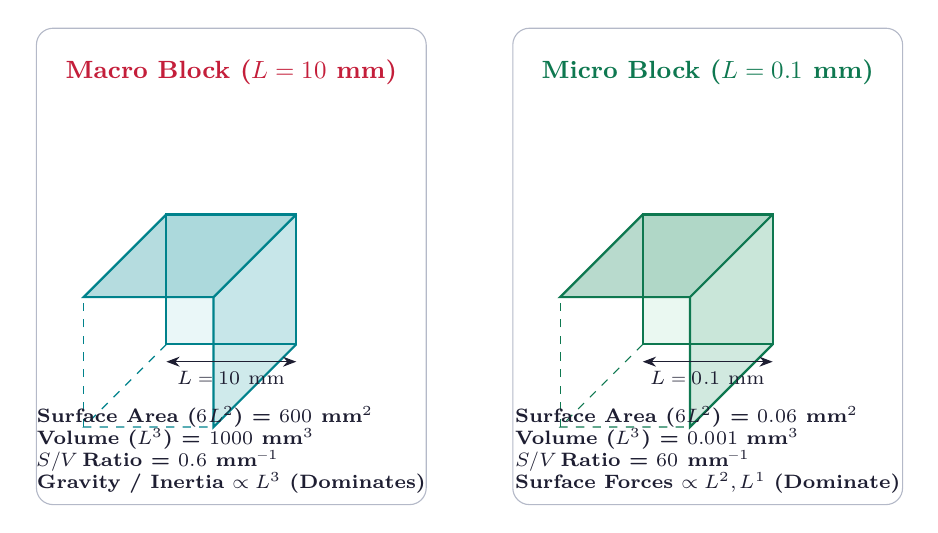
\begin{tikzpicture}[x=0.55cm, y=0.55cm, z=0.35cm, >=Stealth]
  % Card container 1 (Macro-scale)
  \begin{scope}[shift={(-5.5,0)}]
    \draw[fill=white, draw=mgframe, rounded corners=6pt] (-4.5,-5.2) rectangle (4.5,5.8);
    \node[anchor=north, font=\small\bfseries\color{myred}] at (0,5.3) {Macro Block ($L = 10\text{ mm}$)};
    
    % Draw 3D Cube
    \coordinate (O1) at (-1.5,-1.5,0);
    \coordinate (A1) at (1.5,-1.5,0);
    \coordinate (B1) at (1.5,1.5,0);
    \coordinate (C1) at (-1.5,1.5,0);
    \coordinate (D1) at (-1.5,-1.5,-3);
    \coordinate (E1) at (1.5,-1.5,-3);
    \coordinate (F1) at (1.5,1.5,-3);
    \coordinate (G1) at (-1.5,1.5,-3);
    
    \fill[hdrteal, opacity=0.6] (O1) -- (A1) -- (B1) -- (C1) -- cycle;
    \fill[hdrteal!80!myteal, opacity=0.6] (A1) -- (E1) -- (F1) -- (B1) -- cycle;
    \fill[hdrteal!60!myteal, opacity=0.6] (C1) -- (B1) -- (F1) -- (G1) -- cycle;
    
    \draw[myteal, thick] (O1) -- (A1) -- (B1) -- (C1) -- cycle;
    \draw[myteal, thick] (A1) -- (E1) -- (F1) -- (B1);
    \draw[myteal, thick] (C1) -- (G1) -- (F1);
    \draw[myteal, dashed] (O1) -- (D1) -- (E1);
    \draw[myteal, dashed] (D1) -- (G1);
    
    \draw[<->, mydark, thin] ($(O1)-(0,0.4)$) -- ($(A1)-(0,0.4)$) node[midway, below, font=\scriptsize] {$L = 10\text{ mm}$};
    
    \node[anchor=north, align=left, font=\scriptsize\bfseries\color{mydark}] at (0,-2.7) {
      Surface Area ($6L^2$) = $600\text{ mm}^2$ \\
      Volume ($L^3$) = $1000\text{ mm}^3$ \\
      $S/V$ Ratio = $0.6\text{ mm}^{-1}$ \\
      Gravity / Inertia $\propto L^3$ (Dominates)
    };
  \end{scope}

  % Card container 2 (Micro-scale)
  \begin{scope}[shift={(5.5,0)}]
    \draw[fill=white, draw=mgframe, rounded corners=6pt] (-4.5,-5.2) rectangle (4.5,5.8);
    \node[anchor=north, font=\small\bfseries\color{mygreen}] at (0,5.3) {Micro Block ($L = 0.1\text{ mm}$)};
    
    % Draw 3D Cube (visually identical but labeled differently to show scale change)
    \coordinate (O2) at (-1.5,-1.5,0);
    \coordinate (A2) at (1.5,-1.5,0);
    \coordinate (B2) at (1.5,1.5,0);
    \coordinate (C2) at (-1.5,1.5,0);
    \coordinate (D2) at (-1.5,-1.5,-3);
    \coordinate (E2) at (1.5,-1.5,-3);
    \coordinate (F2) at (1.5,1.5,-3);
    \coordinate (G2) at (-1.5,1.5,-3);
    
    \fill[hdrgreen, opacity=0.6] (O2) -- (A2) -- (B2) -- (C2) -- cycle;
    \fill[hdrgreen!80!mygreen, opacity=0.6] (A2) -- (E2) -- (F2) -- (B2) -- cycle;
    \fill[hdrgreen!60!mygreen, opacity=0.6] (C2) -- (B2) -- (F2) -- (G2) -- cycle;
    
    \draw[mygreen, thick] (O2) -- (A2) -- (B2) -- (C2) -- cycle;
    \draw[mygreen, thick] (A2) -- (E2) -- (F2) -- (B2);
    \draw[mygreen, thick] (C2) -- (G2) -- (F2);
    \draw[mygreen, dashed] (O2) -- (D2) -- (E2);
    \draw[mygreen, dashed] (D2) -- (G2);
    
    \draw[<->, mydark, thin] ($(O2)-(0,0.4)$) -- ($(A2)-(0,0.4)$) node[midway, below, font=\scriptsize] {$L = 0.1\text{ mm}$};
    
    \node[anchor=north, align=left, font=\scriptsize\bfseries\color{mydark}] at (0,-2.7) {
      Surface Area ($6L^2$) = $0.06\text{ mm}^2$ \\
      Volume ($L^3$) = $0.001\text{ mm}^3$ \\
      $S/V$ Ratio = $60\text{ mm}^{-1}$ \\
      Surface Forces $\propto L^2, L^1$ (Dominate)
    };
  \end{scope}
\end{tikzpicture}
\end{tcolorbox}

% ===============================================================================
\section{Scaling of Physical Forces}
% ===============================================================================

To design micro-actuators and micro-sensors, we must analyze how different physical forces scale down.

\subsection{Gravity and Inertial Forces}
The mass of an object is $m = \rho V \propto L^3$. The gravitational force is:
$$F_g = m g = \rho V g \propto L^3$$
Scaling factor: $[s^3]$.

\textbf{Inertial Force ($F_i$):} Under constant acceleration $a$, $F_i = m a \propto L^3$. Scaling factor: $[s^3]$.

\textbf{Implication:} As dimensions shrink by $10$ times ($s=0.1$), gravity and inertia drop by $1000$ times. At the micro-scale, gravity becomes negligible. Dust mites can walk on walls because gravitational pull is far weaker than surface adhesion.

\subsection{Electrostatic Force}
For a parallel-plate actuator with plate area $A$, plate separation $d$, and applied voltage $V$:
$$F_e = \frac{1}{2} \frac{\epsilon A V^2}{d^2} \propto \frac{L^2 V^2}{L^2} \propto V^2$$
The scaling behavior depends on how the voltage $V$ is scaled:

\subsubsection{Case A: Constant Voltage Scaling \texorpdfstring{($V \propto L^0$)}{V propto L0}}
If the voltage $V$ remains constant while scaling the physical dimensions ($A \propto L^2$, $d \propto L^1$):
$$F_e \propto \frac{L^2 \cdot (1)^2}{L^2} \propto L^0 = 1$$
Scaling factor: $[s^0]$.

\textbf{Implication:} The electrostatic force remains completely constant as the device scales down. This makes electrostatic actuators highly efficient at small scales.

\subsubsection{Case B: Constant Electric Field Scaling \texorpdfstring{($E = V/d = \text{const} \implies V \propto L^1$)}{E = V/d = const => V propto L1}}
To prevent dielectric breakdown in air, the electric field $E$ must be kept constant, meaning the voltage $V$ is scaled down proportionally with gap distance $d$ ($V \propto L^1$):
$$F_e \propto \frac{L^2 \cdot (L)^2}{L^2} \propto L^2$$
Scaling factor: $[s^2]$.

\textbf{Comparison with Gravity:}
$$\frac{F_e}{F_g} \propto \frac{L^2}{L^3} \propto L^{-1}$$
As $L \to \mu\text{m}$ range, the ratio $\frac{F_e}{F_g}$ becomes extremely large, proving that electrostatic forces are orders of magnitude stronger than gravity at micro-scale.

\subsection{Electromagnetic Force}
For an electromagnetic actuator, the magnetic force on a current-carrying conductor of length $l$ in a magnetic field $B$ is:
$$F_m = I (l \times B) \propto I \cdot L \cdot B$$
Let us assume constant current density $J = I / A_{\text{wire}} = \text{const}$, which implies the current scales as $I \propto A_{\text{wire}} \propto L^2$.
The magnetic field $B$ generated by a micro-coil scales as $B \propto \frac{N I}{L} \propto \frac{1 \cdot L^2}{L} \propto L^1$.
$$F_m \propto (L^2) \cdot (L^1) \cdot (L^1) \propto L^4$$
Scaling factor: $[s^4]$.

If permanent magnets are used where $B \propto L^0$ (constant magnetic flux density):
$$F_m \propto I \cdot L \cdot B \propto (L^2) \cdot (L^1) \cdot (1) \propto L^3$$
Scaling factor: $[s^3]$.

\textbf{Implication:} Magnetic coil forces scale as $L^4$, meaning they disappear extremely fast as scale decreases. Hence, magnetic actuators are rarely used in MEMS, unless permanent magnets are integrated.

\subsection{Surface Tension Force}
Surface tension force acts along the contact perimeter $P$ of a fluid interface:
$$F_s = \gamma P \sin\theta \propto L^1$$
where $\gamma$ is the surface tension coefficient ($N/m$), and $P$ is perimeter ($\propto L^1$).
Scaling factor: $[s^1]$.

\textbf{Comparison with Gravity:}
$$\frac{F_s}{F_g} \propto \frac{L^1}{L^3} \propto L^{-2}$$
At $L = 10\ \mu\text{m}$, surface tension forces are $10^8$ times stronger than gravity. This leads to stiction, where moving micro-structures stick to the substrate during liquid-based etching releases.

% ===============================================================================
\section{Fluidic and Thermal Scaling}
% ===============================================================================

Scaling down also changes heat and fluid transport physics.

\subsection{Fluidic Scaling: Reynolds Number \texorpdfstring{($Re$)}{Re}}
The Reynolds number determines the flow regime (laminar vs. turbulent) of a fluid in a channel:
\begin{tcolorbox}[formulabox, title={Reynolds Number Scaling}]
$$Re = \frac{\rho v D_h}{\mu}$$
where:
\begin{tabular}{lcl}
$\rho$ & = & density of fluid ($kg/m^3$) $\propto L^0$ \\
$v$ & = & flow velocity ($m/s$) $\propto L^0$ (assumed constant) \\
$D_h$ & = & hydraulic diameter of the channel ($m$) $\propto L^1$ \\
$\mu$ & = & dynamic viscosity of fluid ($Pa \cdot s$) $\propto L^0$
\end{tabular}
\end{tcolorbox}
Therefore:
$$Re \propto L^1$$
Scaling factor: $[s^1]$.

\textbf{Physical Consequences in Microfluidics:}
\begin{itemize}[leftmargin=*, itemsep=2.5pt]
  \item In macro-scale pipes, $Re > 4000$ (turbulent flow, dominant inertia).
  \item In micro-channels ($D_h \approx 50\ \mu\text{m}$), $Re \ll 1$ (typically $0.1$ to $10$).
  \item \textbf{Strict Laminar Flow:} At low $Re$, fluid flows in parallel streams without mixing. Turbulent mixing is impossible.
  \item \textbf{Diffusion Mixing:} Mixing occurs only via passive molecular diffusion. The diffusion time $t$ scales as:
  $$t \propto \frac{x^2}{D} \propto L^2$$
  Since the diffusion distance $x \approx L$ is extremely small in micro-channels, mixing by diffusion is fast enough for practical microfluidic applications, despite the laminar regime.
\end{itemize}

\subsection{Thermal Scaling}
Let us analyze heat transfer by conduction through a medium of area $A$, thickness $d \approx L$, and thermal conductivity $k$:
\begin{itemize}[leftmargin=*, itemsep=3.5pt]
  \item \textbf{Heat Conduction Flow Rate ($q$):}
  $$q = -k A \frac{\Delta T}{d} \propto \frac{L^2}{L^1} \propto L^1$$
  Scaling factor: $[s^1]$.
  \item \textbf{Thermal Resistance ($R_{\text{th}}$):}
  $$R_{\text{th}} = \frac{d}{k A} \propto \frac{L}{L^2} \propto L^{-1}$$
  Scaling factor: $[s^{-1}]$.
  \item \textbf{Heat Capacity ($C_{\text{th}}$):}
  $$C_{\text{th}} = m c_p = \rho V c_p \propto L^3$$
  Scaling factor: $[s^3]$.
  \item \textbf{Thermal Time Constant ($\tau_{\text{th}}$):}
  $$\tau_{\text{th}} = R_{\text{th}} C_{\text{th}} \propto L^{-1} \cdot L^3 \propto L^2$$
  Scaling factor: $[s^2]$.
\end{itemize}

\textbf{Implication:}
The thermal time constant scales as $L^2$. If a thermal actuator is scaled down by a factor of 100 ($s = 0.01$):
$$\frac{\tau_{\text{new}}}{\tau_{\text{old}}} = s^2 = 10^{-4}$$
The device heats and cools $10,000$ times faster. MEMS thermal sensors and actuators can operate in the microsecond range, making them highly responsive.

\newpage
% ===============================================================================
% MANDATORY QUICK REVISION PAGE
% ===============================================================================
\begin{center}
  {\large\bfseries\color{myred} Quick Revision --- Module II}\\[3pt]
  {\small\color{mydark} Scaling Effects in Microsystems $|$ PE-EC603A}
\end{center}
\noindent{\color{myred}\rule{\linewidth}{1.2pt}}
\vspace{4pt}

\begin{tcolorbox}[formulabox, title={\textbf{Summary of Scaling Laws}}]
\renewcommand{\arraystretch}{1.3}
\begin{tabularx}{\linewidth}{B{3.8cm} Y Y}
\textbf{Physical Parameter} & \textbf{Formula / Definition} & \textbf{Scaling Exponent ($n$ in $L^n$)} \\
\hline
Surface-to-Volume Ratio & $S/V = 6/L$ & $n = -1$ \\
Gravity / Mass Force & $F_g = \rho V g$ & $n = 3$ \\
Electrostatic Force (Const $V$) & $F_e = \frac{1}{2} \epsilon A V^2 / d^2$ & $n = 0$ \\
Electrostatic Force (Const $E$) & $F_e \propto L^2 E^2$ & $n = 2$ \\
Electromagnetic Force (Coil) & $F_m \propto I L B$ & $n = 4$ \\
Surface Tension Force & $F_s = \gamma P$ & $n = 1$ \\
Reynolds Number & $Re = \rho v D_h / \mu$ & $n = 1$ \\
Thermal Time Constant & $\tau_{\text{th}} = R_{\text{th}} C_{\text{th}}$ & $n = 2$ \\
\end{tabularx}
\end{tcolorbox}

\begin{tcolorbox}[defbox, title={\textbf{One-Line Definitions}}]
\begin{itemize}[leftmargin=*, itemsep=2.5pt, topsep=0pt]
  \item \textbf{Scaling Law:} An equation that predicts how a physical quantity changes when the characteristic size of the system is altered.
  \item \textbf{Surface-to-Volume Ratio ($S/V$):} The ratio of external boundary area to internal volume; it scales as $L^{-1}$ and dominates micro-scale transport.
  \item \textbf{Constant Voltage Scaling:} A micro-scaling method where system voltages are kept constant, resulting in constant electrostatic force ($L^0$).
  \item \textbf{Constant Field Scaling:} A scaling approach where electric field is kept constant to prevent dielectric breakdown, scaling voltage as $L^1$ and force as $L^2$.
  \item \textbf{Reynolds Number ($Re$):} A dimensionless ratio of inertial forces to viscous forces; it scales as $L^1$ and is very small in microsystems.
  \item \textbf{Laminar Flow:} A flow regime characterized by smooth, parallel fluid layers with zero turbulence; occurs when $Re \ll 2000$.
  \item \textbf{Thermal Time Constant ($\tau_{\text{th}}$):} The measure of thermal response speed; scales as $L^2$, enabling microsecond thermal operations in MEMS.
\end{itemize}
\end{tcolorbox}

\begin{tcolorbox}[exambox, title={\textbf{Frequently Asked / Viva Questions}}]
\begin{enumerate}[topsep=0pt, label=\textbf{Q\arabic*.}, itemsep=5pt]
  \item \Q{Why does the surface-to-volume ratio ($S/V$) increase as a device is scaled down?}
    Because surface area scales as $L^2$ while volume scales as $L^3$. Dividing area by volume yields $S/V \propto L^{-1}$, which approaches infinity as $L$ approaches zero.
  \item \Q{Which force dominates: electrostatic or electromagnetic at the micro-scale, and why?}
    Electrostatic force dominates. Under constant voltage scaling, electrostatic force remains constant ($L^0$), whereas magnetic coil forces scale as $L^4$. Thus, electrostatic actuators are vastly superior at the microscale.
  \item \Q{Why is constant voltage scaling preferred over constant field scaling for MEMS actuators?}
    Under constant voltage scaling, the force remains constant ($L^0$). Under constant field scaling, the force drops as $L^2$, reducing performance at smaller sizes.
  \item \Q{What is stiction in surface micromachining and which scaling law causes it?}
    Stiction is the permanent sticking of released micro-beams to the substrate. It is caused by capillary surface tension forces, which scale as $L^1$, dominating gravity ($L^3$) during the wet-release drying process.
  \item \Q{Why is it impossible to create turbulent mixing inside a standard microfluidic channel?}
    Because the hydraulic diameter ($D_h \propto L^1$) is tiny, resulting in a very low Reynolds number ($Re \propto L^1 \ll 1$). At such low values, flow is strictly laminar and turbulence cannot form.
  \item \Q{How do fluids mix in a microfluidic channel if the flow is strictly laminar?}
    Mixing occurs entirely via molecular diffusion. Because diffusion distances are extremely small, diffusion times (which scale as $t \propto L^2$) are short enough to allow rapid mixing.
  \item \Q{Why do MEMS thermal actuators have extremely fast response times?}
    The thermal time constant $\tau_{\text{th}}$ scales as $L^2$. Decreasing dimensions by a factor of 100 reduces the heating/cooling response time by a factor of 10,000.
  \item \Q{How does magnetic force scale for permanent magnets in MEMS?}
    Since the magnetic flux density $B$ of a permanent magnet scales as $L^0$, the force scales as $F_m \propto I L B \propto (L^2)(L^1)(1) \propto L^3$. This is better than coil-based magnetic forces ($L^4$).
  \item \Q{Why do dust particles float in air while stones fall quickly?}
    For a stone (macro-scale), weight ($L^3$) dominates over air resistance ($L^2$). For dust (micro-scale), weight is negligible, and surface drag dominates, keeping the particle suspended.
  \item \Q{Explain the scaling of heat conduction flow rate.}
    According to Fourier's law, heat conduction rate $q = -k A \frac{\Delta T}{d}$. Since area $A \propto L^2$ and distance $d \propto L^1$, the heat flow rate $q$ scales as $L^1$.
  \end{enumerate}
\end{tcolorbox}

\begin{tcolorbox}[tikzbox, title={Actuator Scaling Law Comparison Summary}]
\renewcommand{\arraystretch}{1.45}
\par\noindent
\begin{tabularx}{\linewidth}{|B{3.2cm}|Y|Y|Y|}
\hline
\textbf{Actuation Mode} & \textbf{Scaling Exponent ($n$)} & \textbf{Strength at Macro-scale} & \textbf{Strength at Micro-scale} \\
\hline
\textbf{Electrostatic (Const $V$)} & $n = 0$ (Constant) & Weak (requires high voltages for macro effects). & Very Strong (dominates device behavior). \\
\hline
\textbf{Electrostatic (Const $E$)} & $n = 2$ & Moderate. & Strong. \\
\hline
\textbf{Electromagnetic (Coil)} & $n = 4$ & Very Strong (motors, solenoids). & Extremely Weak (impractical for MEMS). \\
\hline
\textbf{Piezoelectric} & $n = 2$ & Strong. & High force but small stroke. \\
\hline
\textbf{Thermal Bimorph} & $n = 1$ (Speed $\propto L^2$) & Slow. & Extremely Fast, high force. \\
\hline
\end{tabularx}
\tcbset{breakable}
\end{tcolorbox}

\end{document}
